%%%%%%%%%%%%%%%%%%%%%%%%%%%%%%%%%%%%%%%%%
% Journal Article
% LaTeX Template
% Version 1.1 (25/11/12)
%
% This template has been downloaded from:
% http://www.LaTeXTemplates.com
%
% Original author:
% Frits Wenneker (http://www.howtotex.com)
%
% License:
% CC BY-NC-SA 3.0 (http://creativecommons.org/licenses/by-nc-sa/3.0/)
%
%%%%%%%%%%%%%%%%%%%%%%%%%%%%%%%%%%%%%%%%%

%----------------------------------------------------------------------------------------
%	PACKAGES AND OTHER DOCUMENT CONFIGURATIONS
%----------------------------------------------------------------------------------------

\documentclass[twoside]{article}

\usepackage{amsmath}
\usepackage{graphicx}
\usepackage{lipsum} % Package to generate dummy text throughout this template

\usepackage[sc]{mathpazo} % Use the Palatino font
\usepackage[T1]{fontenc} % Use 8-bit encoding that has 256 glyphs
\linespread{1.05} % Line spacing - Palatino needs more space between lines
\usepackage{microtype} % Slightly tweak font spacing for aesthetics

\usepackage[hmarginratio=1:1,top=32mm,columnsep=20pt]{geometry} % Document margins
\usepackage{multicol} % Used for the two-column layout of the document
\usepackage{hyperref} % For hyperlinks in the PDF

\usepackage[hang, small,labelfont=bf,up,textfont=it,up]{caption} % Custom captions under/above floats in tables or figures
\usepackage{booktabs} % Horizontal rules in tables
\usepackage{float} % Required for tables and figures in the multi-column environment - they need to be placed in specific locations with the [H] (e.g. \begin{table}[H])

\usepackage{lettrine} % The lettrine is the first enlarged letter at the beginning of the text
\usepackage{paralist} % Used for the compactitem environment which makes bullet points with less space between them

\usepackage{abstract} % Allows abstract customization
\renewcommand{\abstractnamefont}{\normalfont\bfseries} % Set the "Abstract" text to bold
\renewcommand{\abstracttextfont}{\normalfont\small\itshape} % Set the abstract itself to small italic text

\usepackage{fixltx2e}
\usepackage{caption}
\usepackage{subcaption}

\usepackage{titlesec} % Allows customization of titles
\renewcommand\thesection{\Roman{section}}
\titleformat{\section}[block]{\large\scshape\centering}{\thesection.}{1em}{} % Change the look of the section titles
%----------------------------------------------------------------------------------------
%	TITLE SECTION
%----------------------------------------------------------------------------------------

\title{\vspace{-15mm}\fontsize{14pt}{12pt}\selectfont\textbf{Analyzing the Structure of Knowledge, \\Finding Strongly Connected Components within Wikipedia}} % Article title

\author{
\large
\textsc{Robert Micatka}\\ % Your name
\normalsize University of Michigan \\ % Your institution
}


%----------------------------------------------------------------------------------------

\makeatletter
\newenvironment{tablehere}
  {\def\@captype{table}}
  {}

\newenvironment{figurehere}
  {\def\@captype{figure}}
  {}
\makeatother


\begin{document}


\maketitle 

\date{}

%----------------------------------------------------------------------------------------
%	ABSTRACT
%----------------------------------------------------------------------------------------

\begin{abstract}

	Analyzing multiple wikipedias by finding strongly connected components hints at 
	the underlying structure of information within these collaborative online encylopedias.
	The number and size of the strongly connected components within this database of knowledge 
	will allow the organization to be examined. The number and size of the nodes
	created by the page links will give a clear picture of the macro 
	organizational structure of several different language wikipedias.

 
\end{abstract}

%----------------------------------------------------------------------------------------
%	ARTICLE CONTENTS
%----------------------------------------------------------------------------------------

\begin{multicols}{2} % Two-column layout throughout the main article text

\section{Introduction}

\lettrine[nindent=0em,lines=3]{W} ikipedia is a collaborative, multilingual, open, online 
encyclopedia. Launched on January 15, 2001 by Jimmy Wales and Larry Sanger 
Wikipedia has grown exponentially over the years with the English Wikipedia containing 
over 4.4 million articles and has an estimated 365 million readers annually. \cite{Wikipedia}
Bolstered by these impressive statistics, wikipedia has a very real claim of containing 
nearly the sum total of written human knowledge. Due to the success of the English language
wikipedia hundreds of other languages have spawned their own versions of wikipedia
based on the same foundations.\\

The ability of anyone and everyone to edit Wikipedia is both its greatest strength
and its greatest weakness. The benefit is that experts from all over the world can
edit and update articles in their speciality, allowing articles to be always be up-to-date 
and complete. The downside is the possibility of vandalism. However, there are many
volunteers who keep track of page edits and will quickly revert them if vandalism is 
detected. In addition a 2005 investigation by Nature showed that the science articles 
had a level of accuracy similar to that of Encyclopaedia Britannica. \cite{Nature}

\vfill
\columnbreak

In order to analyze this vast, complex web of data a graph theory technique of
strongly connected components will be utilized. Strongly connected components are
defined as a maximal set of vertices from a directed graph {\it  G} = ({\it  V},{\it E})
where every pair of vertices within the set can are reachable from each other. \cite{Cormen}
Finding strongly connected components within the
directed graph of wikipedia internal page links will allow the structure to be 
uncovered. Finding the strongly connected components will allow identification of
the main nodes of knowledge.\\

In order to find the strongly connected components, after creating the directed graph,
Kosaraju's Algorithm will be utilized. This algorithm uses the transpose of {\it  G} = ({\it  V},{\it E}),
a directed graph, which is defined as {\it  G \textsuperscript{T}} = ({\it  V},{\it E\textsuperscript{T}}). 
This creates what is essentially the same graph but with the directions of the edges reversed.
The generation of the transpose graph allows the strongly connected components
to be computed in linear time using two depth-first searches. The pseudocode for 
the algorithm is as follows: \cite{Cormen}\\

\newpage

Stongly-Connected-Components({\it G})

\begin{enumerate}

\item call DFS({\it G}) to compute finishing times {\it u.f} for each vertex {\it u}

\item compute {\it G \textsuperscript{T}}

\item call DFS({\it G \textsuperscript{T}}), but in the main loop of DFS, consider the vertices
in order of decreasing {\it u.f} (as computed in step 1)

\item output the vertices of each tree in the depth-first forest formed in line 3 as a seperate
strongly connected component

\end{enumerate}

Kosaraju's algorithm is linear-time as the time to create the transpose of {\it G} is
linear in time as well as the two depth-first search passes. This allows for relatively fast
execution time which is needed when working with such large data sets. There are faster
algorithms in practice such as Tarjan's strongly connected components algorithm which only performs
one graph traversal, however,  Kosaraju's is much simpler to implement.



%------------------------------------------------

\section{Methods}

In order to analyze Wikipedia effectively an offline version was required. There are datadumps
and backups taken every couple of weeks for all of the different wikipedias which are available
 to the public for download. The backups consist of a large xml file that constains all of the articles
 as well as internal and external links within the articles. No images are included but are available for download
 as well, however for this project images wererequired. The xml file for the full English wikipedia is on the order of
 44 gigabytes. The major computational hurdle is the resolving the internal links within a wikipedia, using a 3rd party tool
(described below) the full English wikipedia took roughly 16 hours while running on a 6-core machine with 32
GB of RAM. A machine of this calibre was not available to the author. 
Due to these computational limits, smaller wikipedia versions were chosen, namely the Korean, Esperanto, Danish,
Hindi, and Simple English wikipedias. The sizes  (by article count)  of these different wikipedias as well as the English Language 
wikipedia are shown in Table 1.
By choosing smaller wikipedia versions we can (relatively) quickly and easily compare 
the structure of knowledge of the same format between different languages. The multilingual
wikipedias chosen are complete enough to provide useful information while being practically computable.

\begin{tablehere}

\caption{The Size of Different Wikipedias  \cite{wikipediaStatistics}}

\begin{tabular}{| l | l |}

\hline

Wikipedia & \parbox[t]{3cm} {Article Count \\ (thousands)}   \\ \hline

English & 4,400 \\ \hline

Korean & 254 \\ \hline

Esperanto & 188  \\ \hline

Danish & 183 \\ \hline

Hindi & 100 \\ \hline

Simple English & 97  \\ \hline

\end{tabular}

\end{tablehere}

\vspace{10 mm}

The raw data from the xml file is not suitable to creating a directed graph. The internal links must be resolved
in order to show what other pages you can reach from any given page. In order to accomplish this a 3rd party tool
was utilized. Evgeniy Gabrilovich created a tool named wikiprep for his Doctoral thesis work on "Feature Generation for Textual
Information Retrieval Using World Knowledge." \cite{Gabrilovich} Wikiprep parses the xml dump and resolves the internal
links as well as many other tasks that are irrelevant for this project. The new, extended xml file generated
by wikiprep was then parsed and the link information extracted.\\

Using the link information generated by wikiprep a directed graph can be constructed. The links information
contains the node, the article, and its corresponding edges, links to other pages. This graph was 
created using a program written in C++ and stored internally, displaying the graph would not provide
useful context to this examination. Using Kosaraju's algorithm on the created directed graph produced 
a set of strongly connected components. The list of strongly connected
components was reduced by removing all components that consisted of a single node, this occurs
when a node is not part of a strongly connected component, every node is inherently a strongly connected
component by itself.
Removing the singular components does not influence the analysis as nodes linking to themselves are not useful or
interesting in this examination.\\

After the list of strongly connected components was created the size of the components was then found.
Examining the contents of the components would not provide useful contex for this project. Finding the
size of the compenents allows finding the number of components of a similar size. This allows the overall
network structure to be seen as it shows the number of small, medium and large strongly connected
components within wikipedia. This elucidates the overall structure showing many large, more centralized
nodes with more smaller, less connected components on the outskirts.\\

After the sizes of the strongly connected components was determined the lists were then
processed using MATLAB in order to generate a histogram of size frequency. This illustrates the
number of similarily sized nodes within the network.

Note: All code used by this project can be found on my github at \url{https://github.com/s1syphus/ComplexSystems511FinalProject}

%------------------------------------------------

\end{multicols}

\newpage

\section{Results}

%histogram data of the size of strongly connected components
%raw data

\begin{table}[h]

\caption{The Frequency of the Size of Strongly Connected Components within Different Wikipedias}
\centering

\begin{tabular}{| l | l | l | l | l | l |  l | l | l | l | l | l | }

\hline

Wikipedia & 2 & 3 & 4 & 5 & 6 & 7 & 8 & 9 & 10 & {11 - 20} & >20 \\ \hline

Korean & 725 & 198 & 68 & 24 & 9 & 5 & 8 & 2 & 8 & 6 & 1 \\ \hline

Esperanto & 428 & 91 & 31 & 13 & 5 & 1 & 4 & 4 & 5 & 4 & 2 \\ \hline

Danish & 725 & 114 & 34 & 26 & 6 & 4 & 1 & 1 & 4 & 2 & 1 \\ \hline

Hindi & 282 & 62 & 20 & 8 & 2 & 4 & 0 & 1 & 5  & 5 & 2 \\ \hline

Simple English & 293  & 62 & 20 & 10 & 9 & 3 & 3 & 1 & 4 & 3 & 1 \\ \hline


\end{tabular}

\end{table}

\begin{table}[h]

\caption{The Normalized Frequency (percentage) of the Size of Strongly Connected Components within Different Wikipedias}

\centering

\begin{tabular}{| l | l | l | l | l | l |  l | l | l | l | l | l | }

\hline

Wikipedia & 2 & 3 & 4 & 5 & 6 & 7 & 8 & 9 & 10 & {11 - 20} & >20 \\ \hline

Korean & 68.79 & 18.79 & 6.45 & 2.28 & 0.85 & 0.47 & 0.76 & 0.19 & 0.76 & 0.57 & 0.09 \\ \hline

Esperanto & 72.79 & 15.48 & 5.27 & 2.21 & 0.85 & 0.17 & 0.68 & 0.68 & 0.85 & 0.68 & 0.34 \\ \hline

Danish & 78.98 & 12.42 & 3.70 & 2.83 & 0.65 & 0.44 & 0.11 & 0.11 & 0.44 & 0.22 & 0.11 \\ \hline

Hindi & 72.12 & 15.86 & 5.11 & 2.05 & 0.51 & 1.02 & 0 & 0.26 & 1.28  & 1.28 & 0.51 \\ \hline

Simple English & 71.64  & 15.16 & 4.89 & 2.45 & 2.2 & 0.73 & 0.73 & 0.24 & 0.98 & 0.73 & 0.24 \\ \hline

\end{tabular}

\end{table}


\begin{table}[h]
\centering

\caption{Relative Size (percentage) of the Largest Strongly Connected Component in Different Wikipedias \\
	Note: Percentage based on Article count from a different month}

\begin{tabular}{| l | l |}

\hline

Wikipedia & Relative Size (percentage)   \\ \hline

Korean & 107.68 \\ \hline

Esperanto &  95.05  \\ \hline

Danish &  85.30 \\ \hline

Hindi & 34.32 \\ \hline

Simple English & 85.41  \\ \hline

\end{tabular}

\end{table}

\begin{figurehere}
	\centering
	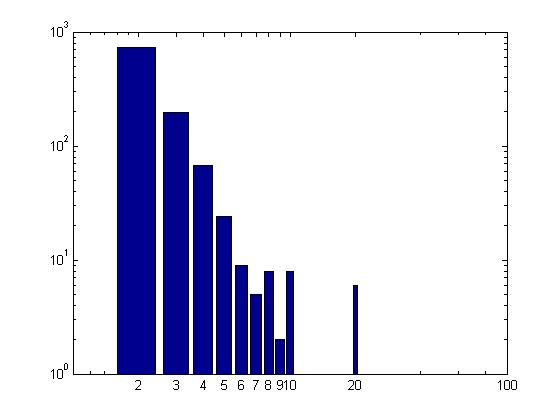
\includegraphics[width=0.5\textwidth]{histogramKo.jpg}
	\caption{Histogram of Frequency of Strongly Connected Component Size for Korean Wikipedia}
	\label{fig:histogramKo}
\end{figurehere}


\begin{figurehere}
	\centering
	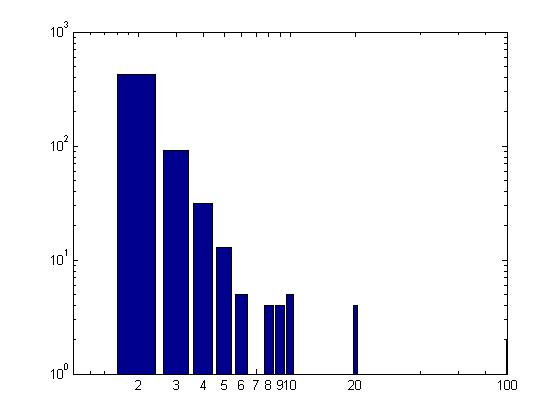
\includegraphics[width=0.5\textwidth]{histogramEo.jpg}
	\caption{Histogram of Frequency of Strongly Connected Component Size for Esperanto Wikipedia}
	\label{fig:histogramEo}
\end{figurehere}

\begin{figurehere}
	\centering
	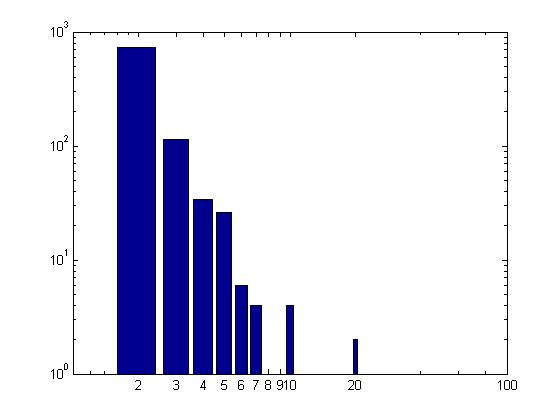
\includegraphics[width=0.5\textwidth]{histogramDa.jpg}
	\caption{Histogram of Frequency of Strongly Connected Component Size for Danish Wikipedia}
	\label{fig:histogramDa}
\end{figurehere}


\begin{figurehere}
	\centering
	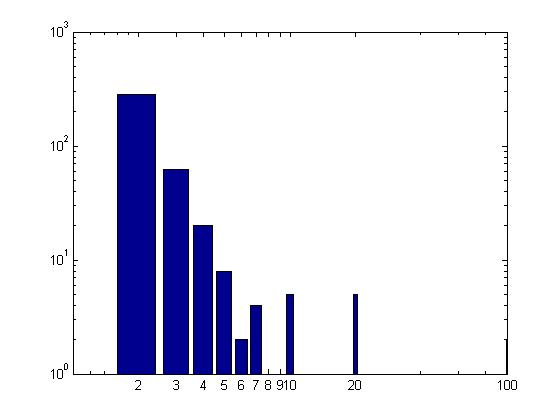
\includegraphics[width=0.5\textwidth]{histogramHi.jpg}
	\caption{Histogram of Frequency of Strongly Connected Component Size for Hindi Wikipedia}
	\label{fig:histogramHi}
\end{figurehere}


\begin{figurehere}
	\centering
	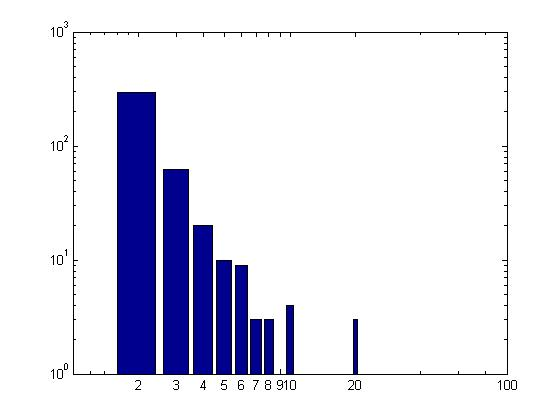
\includegraphics[width=0.5\textwidth]{histogramSE.jpg}
	\caption{Histogram of Frequency of Strongly Connected Component Size for Simple English Wikipedia}
	\label{fig:histogramSE}

\end{figurehere}


%------------------------------------------------

\begin{multicols}{2} % Two-column layout throughout the main article text

\section{Discussion}

The results shown above provide an interesting picture to emerge about the structures of the 
wikipedias examined. All of the wikipedias examined contained one or two massive strongly connected
components that dwarfed all of the others in size. The wikipedias also contained large numbers of 
small strongly connected components ranging from 2 to about 20 nodes in size. When
plotted using a log scale what appears to be a power law emerges. This makes sense on a 
conceptual level as most of the articles within a wikipedia would belong to a single core group, this forms the extremely
large strongly connected component observed. There are also a large number of what are called "orphaned"
components (using the language internal to wikipedia) which are small groups of articles that do not link to 
other articles. \\

The English wikipedia (as well as other language wikipedias) attempt to reduce the number of orphaned 
articles. However, due to the fact that the majority of the edits occur from users, when a page is not seen regularly
it will not be updated and connected appropriately.\\

In addition there was striking similarity in structure between wikipedias
of different languages. This suggests that the structure of knowledge (on a site similar
to wikipedia) is agnostic to language. This is an extremely interesting result which the author can only
speculate on but hints at the underlying structure of how humans categorize and link knowledge together regardless
of language and culture.


\section{Further Study}

Analyzing the five small-to-average sized wikipedias in this project yielded interesting results
about the structure of knowledge accross languages. However, due to computational limits the larger wikipedias, 
those over sevaral thousand articles,
have not been analyzed. Improving the implementation of the algorithms utilized in this project
would allow these larger databases to be analyzed. This would allow the structure of more (and larger)
languages' wikipedias to be examined to see if they fit the pattern described above. Furthermore, 
calculating the power law seen in frequency of the size of the strongly connected components could
provide insight when comparing different languaged wikipedias in the future.\\

 An improvement of the implemenetation of the algorithms utilized 
that could be made would be to parallelize a strongly connected components search algorithm. 
This optimization has been proven to exist with speedups up to ~24x demonstrated. \cite{Parallel} 
This optimization would allow for faster and more efficient computation allowing 
the larger databases to be examined in a timely manner.\\

Once the strongly connected components are found, the next step in understanding the 
structure of the knowledge within wikipedia would be to look at the context of these components.
This could allow the components to be compared to the category tag that is assigned to them
within wikipedia. This comparison would be interesting to see which seemingly different
categories are connected as well as how they are connected.\\


\end{multicols}



%----------------------------------------------------------------------------------------
%	REFERENCE LIST
%----------------------------------------------------------------------------------------

\begin{thebibliography}{99} % Bibliography - this is intentionally simple in this template

\bibitem{Wikipedia} "Wikipedia." {\em Wikipedia.}
		Web. 19 Dec 2013. <\url{http://en.wikipedia.org/wiki/Wikipedia}>.
	
\bibitem{Nature} "Internet Encyclopedias Go Head to Head." {\em Nature}
		(15 Dec 2005). <\url{http://www.nature.com/nature/journal/v438/n7070/full/438900a.html}>.

\bibitem{Gabrilovich} "Wikipedia Preprocessor (Wikiprep)."
	(2 November 2010). <\url{http://www.cs.technion.ac.il/~gabr/resources/code/wikiprep/}>.

\bibitem{Cormen} "Cormen, T., Stein, C., Rivest, R., and Leserson, C." (2009).
	 {\em Introduction to Algorithms.} (3rd ed).
	
\bibitem{Parallel} "Hong, S., Rodia, N., and Olukotun, K." (2013).
	{\em Technical report: On fast parallel detection of strongly connected components (scc) in small-world graphs}.
	(Pervasive Parallelism Laboratory, Stanford University, Stanford, CA).
	Retrieved from <\url{http://ppl.stanford.edu/papers/techreport2013_hong.pdf}>.
	
\bibitem{wikipediaStatistics} "Wikipedia Statistics." {\em Wikipedia Statistics.}
		Web. 20 Dec 2013. <\url{http://stats.wikimedia.org/EN/TablesArticlesTotal.htm}>.



\end{thebibliography}

%----------------------------------------------------------------------------------------



\end{document}
